%%
% このファイルは筑波大学情報学群情報科学類の卒業研究論文のサンプルです。
% このファイルを書き換えて、このサンプルと同様の書式の論文をLaTeXを使って
% 作成できます。
% 
% OSやLaTeXの設定によっては漢字コードや改行コードを変更する必要があります。
%%
\documentclass[a4paper,11pt]{jreport}

%%【PDF, PostScript, JPEG, PNG等の画像の貼り込み】
%% dvipdfmx を使う場合
\usepackage[dvipdfmx]{graphicx}
%% dvipdfmx を使ってPDFの「しおり」を付ける場合
%%\usepackage[dvipdfmx,bookmarks=true,bookmarksnumbered=true,bookmarkstype=toc]{hyperref} \usepackage{pxjahyper}
\usepackage{ulem}
\usepackage{times} % use Times font instead of default one
\usepackage{url}

\setcounter{tocdepth}{3}
\setcounter{page}{-1}

\setlength{\oddsidemargin}{0.1in}
\setlength{\evensidemargin}{0.1in} 
\setlength{\topmargin}{0in}
\setlength{\textwidth}{6in} 
%\setlength{\textheight}{10.1in}
\setlength{\parskip}{0em}
\setlength{\topsep}{0em}

%% タイトル生成用パッケージ(重要)
\usepackage{coins-jp}

%% タイトル
\title{ユーザ空間並列ファイルシステムのための\\システムコールフックライブラリの設計と評価}
%% 著者
\author{宮内 遥楓}
%% 指導教員
\advisor{建部 修見}

%% 年度と主専攻名
\fiscalyear{2024}
%\majorfield{ソフトウェアサイエンス主専攻}
\majorfield{情報システム主専攻}
%\majorfield{知能情報メディア主専攻}

\begin{document}
\maketitle
\thispagestyle{empty}
\newpage

\thispagestyle{empty}
\vspace*{20pt plus 1fil}
\parindent=1zw
\noindent
%%
%% 論文の要旨
%%
\begin{center}
{\Large \bf 要旨}
\vspace{2cm}
\end{center}
ユーザー空間並列ファイルシステムは、ストレージシステムの性能を向上させるために開発されてきた~\cite{tatebe2022chfs, 8514892, 10177390}。 
一方、POSIXインターフェースは、標準として長い間アプリケーションに使用されてきた。 
多くのアプリケーションを動作させるためにはPOSIXインタフェースのサポートが必要であるが、
FUSEやシステムコールインターセプションライブラリなどの既存の手法には様々な問題がある。
本研究では、バイナリ書き換えに基づくシステムコールフック機構であるzpoline~\cite{288689}を利用することでこの問題を解決し、
その性能結果を示す。

%%%%%
\par
\vspace{0pt plus 1fil}
\newpage

\pagenumbering{roman} % I, II, III, IV 
\tableofcontents
\listoffigures
%\listoftables

\pagebreak \setcounter{page}{1}
\pagenumbering{arabic} % 1,2,3

\chapter{序論}

論文は序論で開始し、最終章は結論で終える。序論には論文全体の見通し・何が
研究の要点であるか・何に焦点を当てて研究を行うか等、この章を読めば論文の
分野・内容が大筋で掴めるように書く。

研究の内容や分野によっては書き方が異なる場合もあるので、詳しいことは指導
教員に聞くとよい。この文書は主にスタイルの作成方法と、論文の体裁を示すの
みであり、どうやったらよい論文になるかの示唆は含まれていない。

\chapter{背景}

\section{ファイルシステム}

\section{ユーザ空間ファイルシステム}

\section{並列ファイルシステム}

\chapter{システムコールフックライブラリの設計}

\section{zpoline}

\section{CHFS}

\chapter{既存手法}
アプリケーションの書き換えなしでユーザ空間ファイルシステムを利用する方法は大きく分けて2つある.
\section{FUSE}
FUSE(Filesystem in Userspace)はユーザ空間ファイルシステムを開発するときに最もメジャーなフレームワークである. FUSEを利用することで
容易にユーザ空間ファイルシステムをPOSIXインターフェースに対応させることができるため, SSHFS\cite{hoskins2006sshfs}, GlusterFS\cite{davies2013scale}, 
ZFS\cite{rodeh2003zfs}など数多くのFUSEベースのファイルシステムが開発されている.

しかしながら,アプリケーションとFUSEプロセスとの通信コストや,コンテキストスイッチによるオーバーヘッドが原因の性能低下により, 
特にパフォーマンスが求められる高性能計算分野での利用は適していないと論じられている\cite{brinkmann2020ad}. 

アプリケーションがFUSEを介してユーザ空間ファイルシステムにアクセスする過程を\figurename~\ref{fig:FUSE}に示す. アプリケーションが
標準ライブラリを通じてシステムコールを発行し, VFSに到達するまでは通常のファイルシステムアクセスと同じである. 

TODO: FUSEの説明追加

\newpage


\begin{figure}[h]
	\begin{minipage}[b]{1\columnwidth}
		\centering
		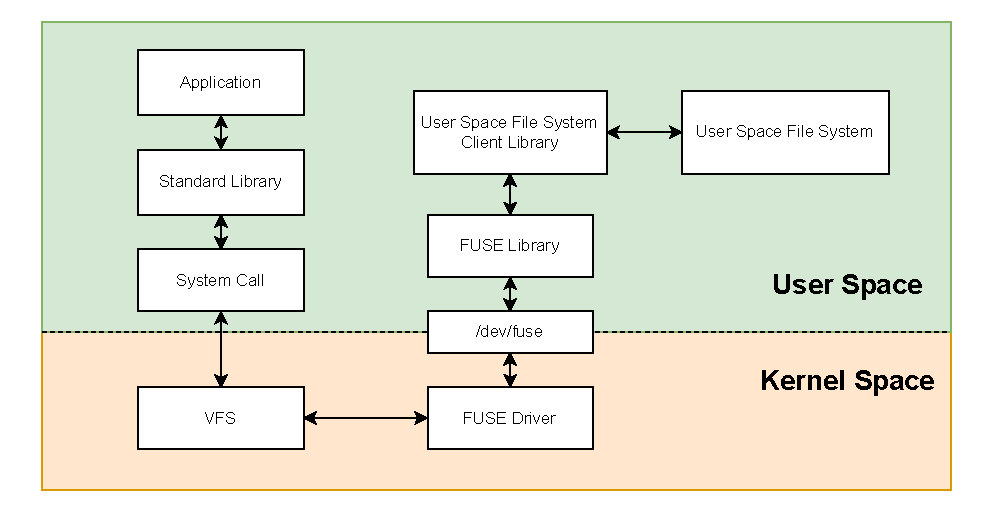
\includegraphics[width=0.9\linewidth]{./figure/FUSE.pdf}
		\caption{FUSE アーキテクチャ}
		\label{fig:FUSE}
	\end{minipage}
\end{figure}

\newpage


\section{プリロードライブラリ}
libsysio
syscall\_intercept
gotcha

\chapter{評価実験}
前章で実装したシステムコールライブラリの評価実験を行う。本実験の目的としては、ユーザ空間ファイルシステムが提供する
クライアントライブラリを使用した場合と比べてどの程度ストレージアクセス性能が保たれるか評価すること、また既存手法の中で
最もよく用いられるFUSEとの性能を比較することである。

\section{実験環境}
実験環境として筑波大学計算科学研究センターが運用するPegasusスーパーコンピュータを利用する。Pegasusは各計算ノードに専用のストレージを
保持しており、SSDとPMEMを利用できる。本実験ではPMEMをdevdaxモードで利用する。計算ノード間はInfiniBand NDR 200で接続されており、
帯域幅は200Gbpsである。
\section{実験方法}
本実験ではIORベンチマーク\cite{ior}を実行してCHFSファイルシステムに対するファイル読み込み/書き込み帯域幅を測定する。提案手法を含む
以下の3種類の条件下でベンチマークを実行し、その性能を比較する。

\subsection{ネイティブAPI}
ファイルシステムが提供するクライアントライブラリのAPIを利用してファイルにアクセスする。具体的にはIORベンチマークのソースコードを変更し、
CHFSクライアントライブラリの関数を呼び出すことでCHFS上のファイルへの読み書きを行う。
\subsection{FUSE}
CHFSサーバを起動した後、chfuseコマンドを使用して指定のディレクトリにマウントする。IORベンチマークのファイル読み込み・書き込みは
マウントしたディレクトリに対して実行する。
\subsection{システムコールフック(提案手法)}
前章で実装したシステムコールフックライブラリを利用する。仮想的なマウントディレクトリ/chfsに対してIORベンチマークのファイル読み込み・
書き込みを行う。
\section{実験設定}
Pegasusシステムにおいて、計算ノード10台をCHFSサーバとして割り当て、さらに1台をIORベンチマークの実行に使用し、合計で11台の計算ノードを
専有する。

CHFSはチャンクサイズを16MiBに設定し、各ノード46プロセスでCHFSサーバを起動する。通信プロトコルにverbs、バックエンドにpmemkvを利用する。

IORはプロセス数を1、2、4、…と16まで増やしながら実行する。IORではfile-per-process方式でアクセスし、各プロセスが別々のファイルに
対して1TiB読み書きする。この操作を5回行い、帯域幅の平均を求める。
\section{結果}

実験結果を\figurename~\ref{fig:Evaluation read}と\figurename~\ref{fig:Evaluation write}に示す。どの条件でもプロセス数を増やすに
つれ帯域幅が増加していることがわかる。読み込みの16プロセスにおいて性能の増加がないのは、Pegasus計算ノード間の通信帯域幅200Gbpsに
到達していると考えられる。

基準であるネイティブAPIを使用した場合の性能に対して、提案手法のシステムコールフックは読み込み・書き込みともに同程度の性能を示した。
またFUSEを使用した場合と比較して提案手法は5.3倍から6.4倍高い性能を示した。

\newpage

\begin{figure}[h]
	\begin{minipage}[b]{1\columnwidth}
		\centering
		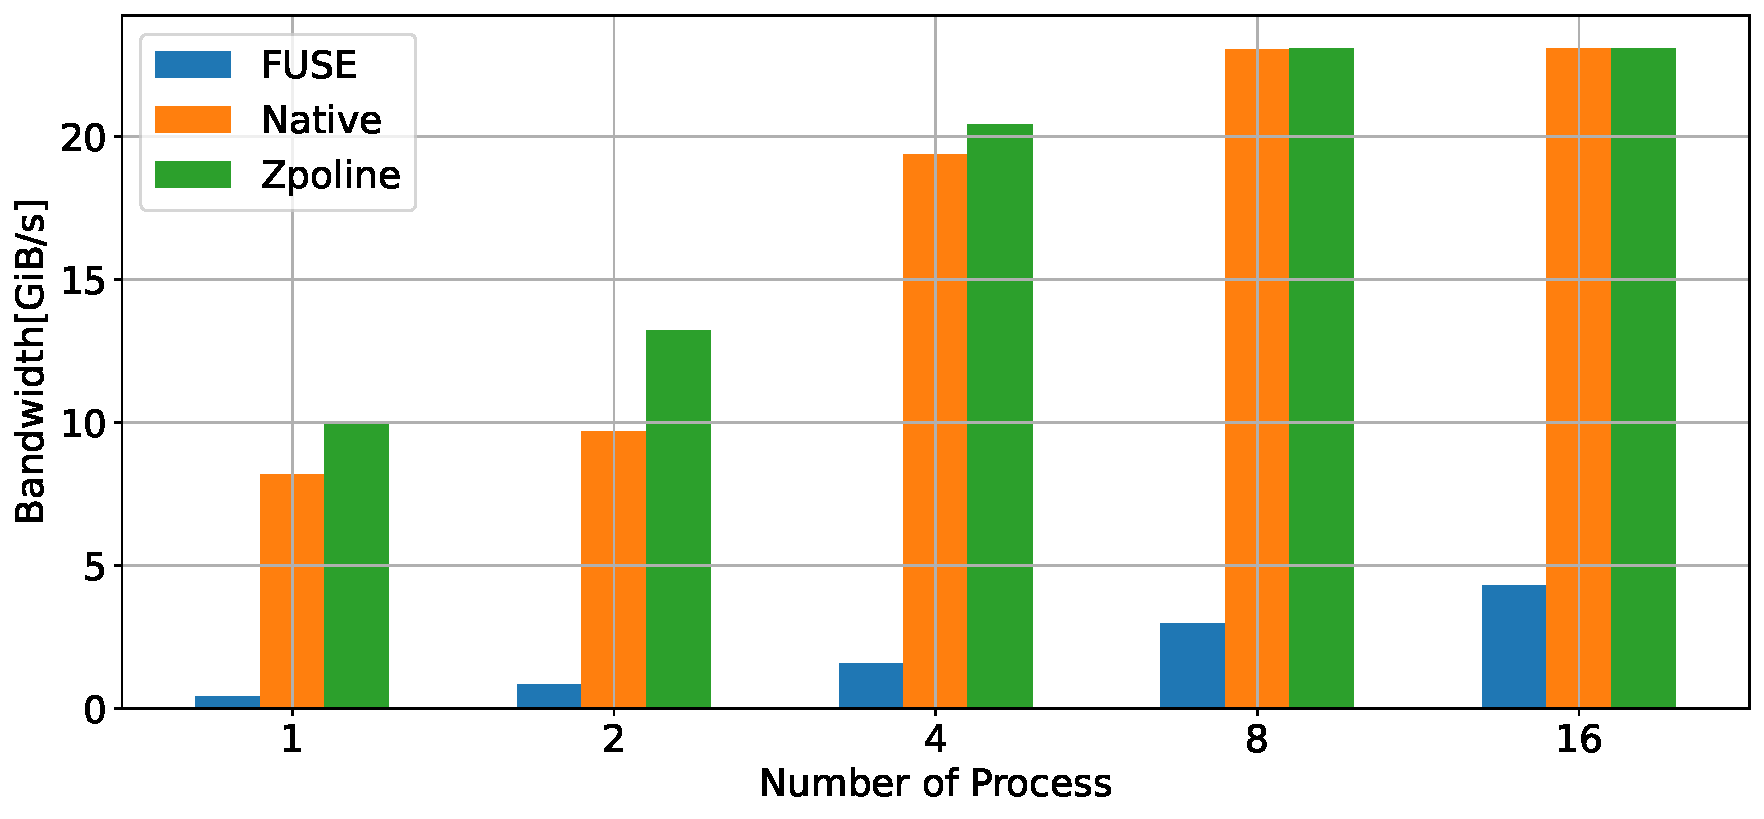
\includegraphics[width=0.9\linewidth]{./figure/ior_benchmark_read.pdf}
		\caption{IOR 読込み性能}
		\label{fig:Evaluation read}
	\end{minipage}
\end{figure}

\begin{figure}[h]
    \begin{minipage}[b]{1\columnwidth}
		\centering
		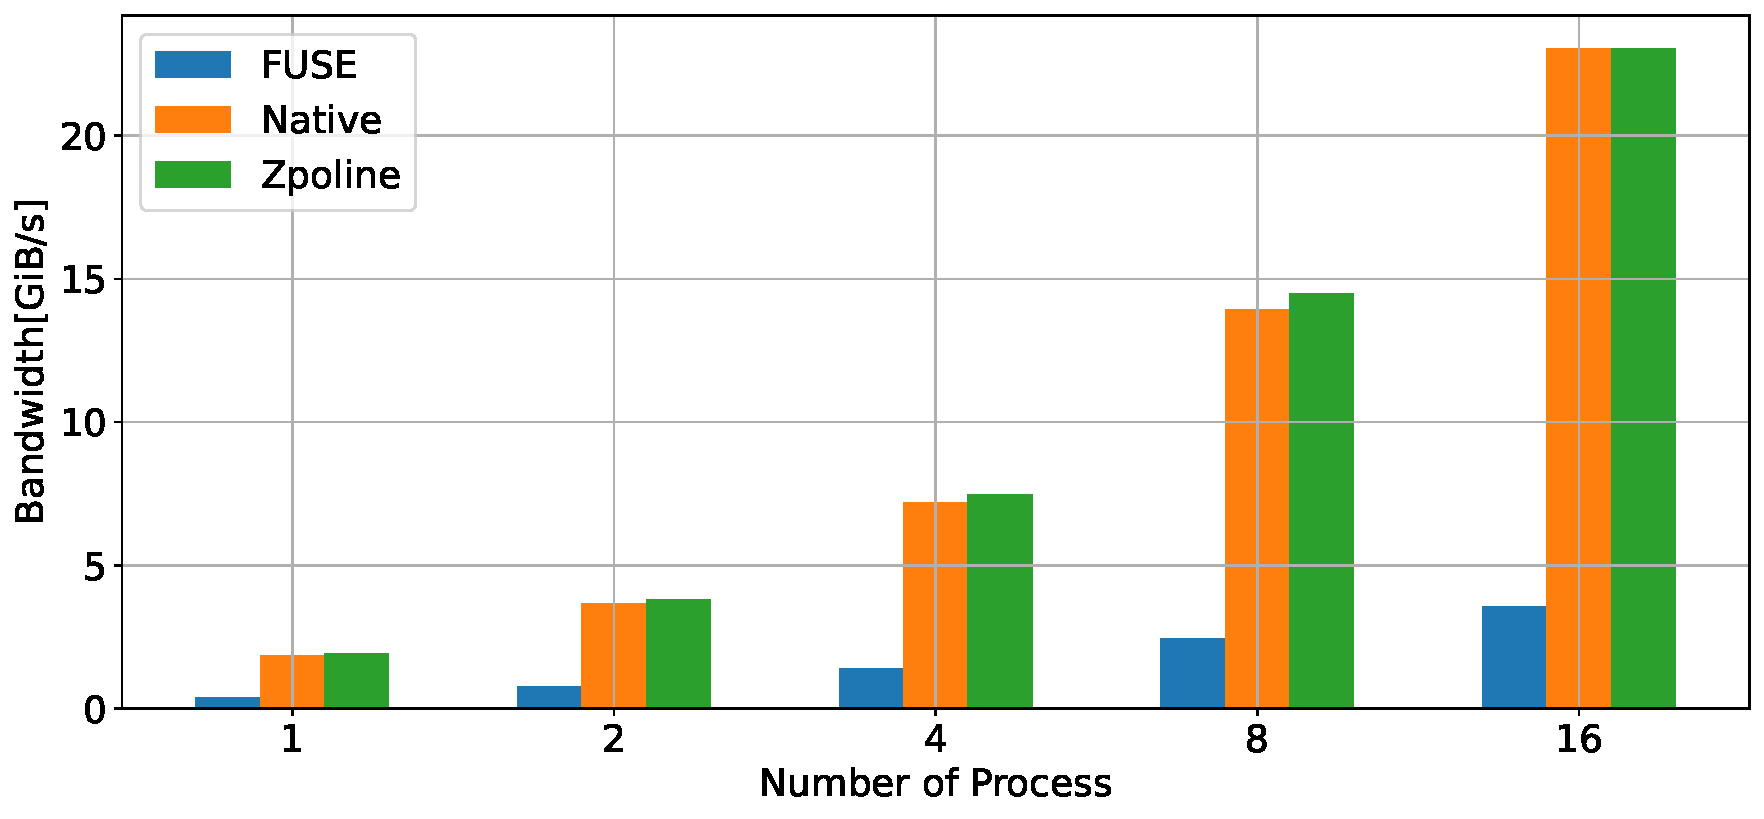
\includegraphics[width=0.9\linewidth]{./figure/ior_benchmark_write.pdf}
		\caption{IOR 書込み性能}
		\label{fig:Evaluation write}
	\end{minipage}
\end{figure}

\chapter{終論}

\chapter*{謝辞}
\addcontentsline{toc}{chapter}{\numberline{}謝辞}
1年間親身かつ丁寧に研究を指導してくださった筑波大学計算科学研究センターの建部修見教授に深く感謝申し上げます。
加えて、研究テーマの相談段階から論文作成にいたるまで研究にご指導ご尽力いただき、また国際会議の発表において共著者として
ご協力いただいたHPCS研究室の小山創平氏に大変感謝申し上げます。
また、計算科学研究センターの研究員である平賀弘平氏、HPCS研究室の杉原航平氏にも研究を進めるうえで多大なアドバイスをいただきました。感謝申し上げます。
同時に、計算科学研究センターの職員の皆様、特に同センター秘書の桑野洋子氏には事務的な面で研究をサポートしていただきありがとうございました。
HPCS研究室の皆様には、研究を進めるにあたり議論を通じてご協力いただきました。
そして共同研究先である富士通研究所の皆様には学外としての立場から大変ありがたいご支援をいただきました。ありがとうございました。
最後に、これまで大学生活を共にした友人と、学生生活を支えてくれた家族に心から感謝致します。

\newpage

\addcontentsline{toc}{chapter}{\numberline{}参考文献}
\renewcommand{\bibname}{参考文献}

\bibliography{main}
\bibliographystyle{junsrt}

\end{document}
